% !TEX TS-program = pdflatex
% !TEX encoding = UTF-8 Unicode

% This is a simple template for a LaTeX document using the "article" class.
% See "book", "report", "letter" for other types of document.

\documentclass[11pt]{article} % use larger type; default would be 10pt
\usepackage{natbib}
\usepackage{mathtools}
\usepackage{graphicx}
\usepackage[colorlinks]{hyperref}
\usepackage[colorinlistoftodos, textwidth=4cm, shadow]{todonotes}

% makes paragraphs have no identation and a space between them
\usepackage{parskip} 


% text coloring
\usepackage{color}

% color definitions

\definecolor{blue}{RGB}{0,0,255}
\definecolor{green}{RGB}{0,255,0}
\definecolor{purple}{RGB}{204,0,102}

% code snippet colors
\definecolor{dkgreen}{rgb}{0,0.6,0}
\definecolor{gray}{rgb}{0.5,0.5,0.5}
\definecolor{mauve}{rgb}{0.58,0,0.82}



% package for code snippets
\usepackage{listings}

% code snippet configuration for haskell
\lstset{frame=tb,
  language=Haskell,
  aboveskip=3mm,
  belowskip=3mm,
  showstringspaces=false,
  columns=flexible,
  basicstyle={\small\ttfamily},
  numbers=none,
  numberstyle=\tiny\color{gray},
  keywordstyle=\color{blue},
  commentstyle=\color{dkgreen},
  stringstyle=\color{mauve},
  breaklines=true,
  breakatwhitespace=true
  tabsize=3
}

\usepackage[utf8]{inputenc} % set input encoding (not needed with XeLaTeX)


%%% Examples of Article customizations
% These packages are optional, depending whether you want the features they provide.
% See the LaTeX Companion or other references for full information.

%%% PAGE DIMENSIONS
\usepackage{geometry} % to change the page dimensions
\geometry{a4paper} % or letterpaper (US) or a5paper or....
% \geometry{margin=2in} % for example, change the margins to 2 inches all round
% \geometry{landscape} % set up the page for landscape
%   read geometry.pdf for detailed page layout information

\usepackage{graphicx} % support the \includegraphics command and options
\graphicspath{ {Graphics/} }
\usepackage{subfigure}

% \usepackage[parfill]{parskip} % Activate to begin paragraphs with an empty line rather than an indent

%%% PACKAGES
\usepackage{booktabs} % for much better looking tables
\usepackage{array} % for better arrays (eg matrices) in maths
\usepackage{paralist} % very flexible & customisable lists (eg. enumerate/itemize, etc.)
\usepackage{verbatim} % adds environment for commenting out blocks of text & for better verbatim
%\usepackage{subfig} % make it possible to include more than one captioned figure/table in a single float
% These packages are all incorporated in the memoir class to one degree or another...

%%% HEADERS & FOOTERS
\usepackage{fancyhdr} % This should be set AFTER setting up the page geometry
\pagestyle{fancy} % options: empty , plain , fancy
\renewcommand{\headrulewidth}{0pt} % customise the layout...
\lhead{}\chead{}\rhead{}
\lfoot{}\cfoot{\thepage}\rfoot{}

%%% SECTION TITLE APPEARANCE
\usepackage{sectsty}
\allsectionsfont{\sffamily\mdseries\upshape} % (See the fntguide.pdf for font help)
% (This matches ConTeXt defaults)

%%% ToC (table of contents) APPEARANCE
\usepackage[nottoc,notlof,notlot]{tocbibind} % Put the bibliography in the ToC
\usepackage[titles,subfigure]{tocloft} % Alter the style of the Table of Contents
\renewcommand{\cftsecfont}{\rmfamily\mdseries\upshape}
\renewcommand{\cftsecpagefont}{\rmfamily\mdseries\upshape} % No bold!

%%% END Article customizations

\newcommand{\projectName}{BitSmuggler }

\title{Report \\ \projectName- Bittorrent camouflage for Tor traffic}
\author{Dan Cristian Octavian}
%\date{} % Activate to display a given date or no date (if empty),
         % otherwise the current date is printed 

\begin{document}

\newcommand{\myparagraph}[1]{\paragraph{#1}\mbox{}\\}
\maketitle

\listoftodos

\tableofcontents

\newpage


%%%%%%%%%%%%%%%%%%%
%%%%% INTRODUCTION %%%%%

\section{Introduction}

\subsection{Problem}

\todo[inline]{change the intorduction according to simon peyton jones's suggestions: a problem statement with an example + achievements}

 “If you have something that you don’t want anyone to know, maybe you shouldn’t be doing it in the first place”. Now, wouldn’t you hire the guy who said this to manage the surveillance system in your totalitarian state? I would, but you better prepare a fat paycheck because he’s the ex-CEO of Google. We are in a time when there’s a lot of talk about privacy and anonymity, because we are in a time where these things are becoming increasingly hard to attain. Most choose not to care, since all is good for the moment, and find the above quote comforting. A few find it alarming, though, because of its impactful indirect implications.

There’s an old book written by a Chinese general, called Sun Tzu, full of reasonable advice about to conduct warfare and, unsurprisingly, a lot of his advice is about how having correct information about your opponent and depriving him of it is the key to victory. Wartime or not, having access to information and the ability to manipulate it and analyze it grants you great power. One would argue that a state’s secret services will use this power to protect its citizens. But once you build a tool that gives you such power, it’s also easy to abuse it or let it slip in the wrong hands.

Since 1988, China has been operating a censorship and surveillance system, codenamed Golden Shield which censors Internet access, observes communications to enforce its totalitarian laws thus depriving its citizens’ of their basic human rights. It is today’s most significant example of things gone wrong with information power tools. Similar situations can be found in Iran or Syria. All these states resort to building censorship and surveillance firewalls, monitoring and manipulating communications between endpoints in their country and the outside.

The problem at hand is of findings ways around these censorship and surveillance systems, to allow people subject to them to access the internet freely and not get caught in the process. Simple solutions such as proxies and VPNs are no longer viable and more sophisticated methods are required. 

This project’s aim is to build a solution to this problem that integrates with the anonymity network Tor by allowing censored users to access the Internet through Tor and avoiding firewall detection by camouflaging Tor traffic as Bittorrent traffic. The idea is to find a cover traffic that goes undetected by filters, has a good throughput and is unlikely to be blocked.

Using Bittorrent traffic as a cover is a promising choice since it is the most prevalent protocol when it come down to upstream traffic and overall the 3nd most prevalent after HTTP and video streaming (in terms of volume of data) ([1] Sandvine, 2013). it has the property that it has a large throughput both downstream and upstream and transports content fit for steganography (eg. video files). Its popularity makes it unlikely to be a target of blocking and doing so would be considered an extreme measure.

The project seeks to also address the issue of Tor proxies using this cover channel being actively probed by scanners seeking to blacklist them through the use of a secret token presented as proof the the client contacting the proxy is to be trusted.
\subsubsection{Contributions}




\subsection{Report Outline}
\todo[inline]{Describe report outline}%

\newpage
%%%%%%%%%%%%%%%%%%
%%%%%BACKGROUND%%%%%
\section{Background}

This section covers the information needed to understand this project, assuming no prior w to knowledge about anonymity networks and censorship circumvention schemes but general knowledge about networks and encryption.

I am going to discuss the following topics:

\begin{itemize}
\item the Tor anonymity network - how it works, what is its purpose
\item surveillance and censorship firewalls - case studies of censorship firewalls in China and Iran 
\item Tor censorship circumvention schemes - what mechanisms does Tor currently provide for defeating the above mentioned firewalls
\item the need for a better tor traffic camouflage
\end{itemize}

%% Sound %%
\subsection{The Tor anonymity network}
Tor is a an anonymity network and a software that allows its users to defend against traffic analysis, a network surveillance technique meant to gather information about a user’s online activity. By using Tor, an individual achieves online anonymity. ([2] Tor project, 2014)

\subsubsection{Purpose}
Why would one need such a service? Suppose you are interested in accessing a website which is blocked by your ISP (ex. Pirate Bay). On the wild side, suppose you are government worker in an oppressive state and want to play the whistleblower role and contact outsiders to reveal secret information, action which could compromise your personal safety. Tor is an appropriate tool for this kind communication since it allows you to keep your communication anonymous: eavesdroppers will not be able to know who you are contacting over the network and your destination cannot know who you are either.

What does Tor effectively offer to users? Why does one need more security than that offered by encryption? It is because encryption hides the data payload of internet packets, while the headers of the packets are visible to any eavesdropper in the network. The packet headers reveal source, destination, size and timing. Tor allows a user to hide this information as well. The receivers of the packets themselves do not know the sender identity either.

Understanding adversary capabilities and intentions gives a more clear image of what privacy protection problems Tor is trying to solve. A traffic analyzer may spy by just sitting somewhere between the source and the destination of the package and observe the packet headers to learn about information exchanges between the parties. It may be more sophisticated and observe multiple parts of the Internet and throw in statistical analysis to track the communications of individuals/organizations.

\subsubsection{How it works}

To understand how Tor works, it is useful to think of it as trying to hide from someone who is following you by using a convoluted path and covering your tracks. Thus, when communicating through Tor, your data follows a random path, moving from one Tor network node to another until it reaches its destination.

Data packets travel from source to destination through the Tor network on what is called a circuit. A circuit is composed of a chain of relays (machines which are part of the Tor network). Each relay in the circuit knows only about the relay before it and the one after it. Thus none of them know the entire path of the data they are transporting. A different set of encryption keys is negotiated by the client for each hop in the circuit so that no relay in the chain can track communications flowing through it. 

The above techniques ensure that an eavesdropper sitting between any 2 relays in a circuit cannot deduce any of the information normally given away by headers. Eavesdropping right at the source or right at the destination only reveals that some unknown packet is going into Tor or some unknown packet is exiting Tor, respectively.

The nodes which compose the Tor network are run entirely by volunteers and the diversity of these volunteers is another aspects which works to enforce the privacy guarantees of Tor. Since Tor nodes are spread across the globe and belong to a series of individuals/organizations and every communication through Tor follows a circuit composed of multiple relays, it is very difficult for one entity to be able to monitor the users of Tor.

\subsubsection{Issues and potential attacks}

However, one can argue that Tor security guarantees may be compromised by an adversary who owns a large amount of nodes in the Tor network or who monitors traffic going into and exiting the network to make statistical correlations. This is an acknowledged weakness of the system and it is a an accepted fact that Tor cannot face a state-level adversary with large resources and great reach. Despite this Tor has a large array of use cases. For example, using Tor to run a criminal organization and hide from the US government is an approach doomed to failure due to their computational and monitoring capabilities. An adversary such as the US has the resources to analyze the network and the influence necessary to monitor the Internet traffic in a variety of places, perhaps outside its national borders.

Much research has gone in evaluating the effectiveness of traffic correlation attacks on the Tor network, which can be put to use as described above. The most recent paper on the subject is the most authoritative ([3] Aaron Johnson, 2013) and it reveals that this attack is more potent than previously believed. The authors develop a framework for analyzing the vulnerability of Tor against attackers owning IXP coalitions or/and being part of the actual network.

\subsubsection{Tor as a censorship circumvention tool}

An interesting use case of Tor is that of using it a censorship and surveillance circumvention tool in countries where Internet access is subject to surveillance such as China and Iran. One could argue that this is a situation where the Tor network is facing a state level adversary and the effort is futile. However, these states tend to be isolated islands to the rest of the world which opposes their policies. This kind of adversary is limited to performing traffic analysis on all incoming and outgoing national traffic, having not much reach outside its borders. Therefore the problem of using Tor to bypass surveillance is reduced to that of finding a way of penetrating their firewall.
A central element of Tor censorship circumvention tools is the Tor bridge. Currently all Tor relays are publicly available. Any censoring adversary who wants to prevent the use of Tor could trivially block access to these machines. That is why there exists a set of Tor nodes which are not publicly available and their addresses can only be obtained through other methods such as providing proof life or communicating with the owner of the bridge. 


\subsection{Surveillance and Censorship firewalls}

The problem at hand is that of developing a mechanism for allowing people to bypass internet surveillance and censorship systems, as part of  the Tor project. This means that such a mechanism aims to defeat a black-box adversary whose resources and techniques are unknown but can be intelligently estimated/guessed. In this section I will go over the necessary background knowledge about this adversary, focusing mostly on China, the owner of the most sophisticated Internet censorship system in the world ([4] OpenNet, 2013), and briefly discussing others such as Iran.

\subsubsection{Observations}

The adversaries aim to inspect information flowing in and out of the state they are operating in, tamper with it and block it as they see fit. They are interested in seeing which are the parties involved in the information exchange, and even though the actual content may be protected by encryption, data about source, destination, timing, size is easily accessible. Furthermore, they have passive and active systems which aim to defeat surveillance and censorship circumvention mechanisms, such as Tor. All of this is achieved by China with the Golden Shield Project (also known as the Great Firewall of China - GFW). ([5] HikingGFW, 2013)

For the purpose of censorship, adversaries employ a series of methods ([6] Zittrain and Eldman, 2003):

\begin{itemize}
\item filter based web server IP address - access to certain IP addresses is denied. All IP based protocols are affected. This is implemented most likely with block lists loaded onto border routers
\item filtering based on DNS IP address - access to DNS servers with certain IPs is denied. May be easier to circumvent if the user has the IP of his target webserver and does not require a name resolution. Most likely uses the same implementation as above.
\item DNS redirection - DNS servers in China resolve domain names to web server addresses other than the official ones ([10] Lowe, 2007)
\item filtering based on keywords in the URL - requests are blocked whenever the URLs contain certain keywords. This is most likely implemented with packet-filtering systems integrated with the border routers.
\item filtering based on keywords present in the HTML response - packets are blocked based on the content of the response. This is a strong argument for the presence a packet filtering system.
\end{itemize}

It was shown that the GFW employs techniques that may be easy to circumvent but the circumvention will not go unnoticed - which highlights an important goal of this project: bypassing the firewalls should go unnoticed. The paper “Ignoring the great firewall a China” ([7] Clayton,  2006) features an experiment which proves that GFW attempts to kill an undesired connection by sending forged TCP reset packets both ways. The authors were speculating that it uses an offline packet analysis system to decide whether a connection is to be dropped or not. Both parties could theoretically choose to ignore the reset message and continue the exchange. However, the surveillance system could easily log this event and pursue an investigation on the communication endpoint located in China.

To circumvent the censorship methods, the most natural tactic is to use a VPN or proxy. However, this is no longer a viable alternative. VPN connections are often now blocked ([8] The Guardian, 2012) which proves GFW is detecting and then killing connections to VPNs or proxies ([5] HikingGFW, 2013). Circumvention tools based on proxies (Ultrasurf, Psiphon) now need to rotate IPs constantly since their servers are continuously blocked. It is very likely that the Golden Shield Project developed tools for detecting VPN, SSH, TLS/SSL traffic and also explicitly analyzes circumvention tools in order to fingerprint their traffic so that they can block them.

According to the paper “How the great Firewall of China is blocking Tor” ([9] Winter, 2012) the GFW is taking strong measures to prevent the use of Tor by its citizens. This is the most extensive study on the issue of Tor blocking in China. Apart from the most obvious measures such as blocking all public relay addresses and all web servers associated with the Tor project, GFW is blocking the Tor bridges as well. For example, the pool of bridges which are obtained by providing proof of life (captcha solving) on a Tor website is blocked entirely. 

Moreover, their experiment, which involved pretending to be a tor client in China, showed GFW is actively probing machines on the web to see if they are Tor bridges. The authors conjectured that DPI (deep packet inspection) boxes are being used to discover packets that are potentially tor packets. Suspect network connections get their addresses placed in a queue. These addresses are later automatically scanned by connecting to them through the Tor protocol. If the machines respond as a Tor bridge would, they are blocked.

Based on the study of the IPs of the Tor bridge scanners, the authors were lead to believe that an IP spoofing scheme is used to hide the origin of the scanners. Therefore, any attempt to distinguish between an honest IP and a scanner IP based on the address alone is unlikely to succeed. 

The speculated surveillance systems described above seemed to have flaws and peculiarities: some Tor relay directories were not blocked, some tor bridges never got blocked or got unblocked after a while after exhibiting tor activity. Nonetheless, an intent to minimize collateral damage was observed, since undesired connections were dropped for (address, port) tuples meaning IPs weren’t blocked entirely.  My belief is that in searching for a solid solution, one cannot rely on these small failures or indulgences. They can be exploited for short term gains, but a real solution to the problem should assume an adversary which has the above capabilities perfected.

\subsubsection{Adversary sketch}

Given the all the information gathered when reverse engineering the GFW and assuming an adversary with vast resources I am sketching the model of the adversary in the following way:

\begin{itemize}
\item has the capability of observing all traffic exiting and entering its national borders
\item has complete control over its internal network infrastructure from ISPs to DNS servers, being capable  of techniques such as IP spoofing
\item all packets it observes can be subject to DPI 
\item it has the ability to run sophisticated statistical analysis at a large scale
\item it has active probing capabilities 
\item it is willing to block large amounts of traffic and important Internet players (eg. China blocked Google on numerous occasions)
\item its automated computations can be augmented by Mechanical Turk - style human supported task solving systems (eg. to solve a large number of captchas)
\item it has the authority to inspect all the machines on its national territory
\item the adversary draws great value from merely finding out the 2 parties involved in an exchange and not necessarily blocking; based on this information it can take the investigation forward and 
\item interacting with it is analogous to examining a quantum state, in the sense that the observation affects the outcome. For example, running experiments to test the effectiveness of circumvention techniques may trigger defensive responses on the part of the adversary.
\item it is very hard to prove the effectiveness of a technique against it since merely getting data across its firewall is not a proof of success - the adversary may have the capability to block but it might just be observing silently
\item changes to the infrastructure tend to be quite slow and expensive since they happen at the level of a huge state
\end{itemize}

\subsection{Existing solutions}

This section covers the existing techniques for solving the problem at hand, discussing the ones provided by Tor, companies and other open initiatives.
 
Since traditional VPN/proxy based solutions are quickly becoming obsolete due to the adversary blocking such connections, more sophisticated systems have been developed using techniques various techniques such as large numbers of rotating changing proxies, hidden proxies shared through more secure channels (Tor bridges) and traffic obfuscation/camouflage.

\subsubsection{Private company solutions}
Censorship circumvention solutions developed by companies deserve attention, even though they are often overlooked in the papers from the research community. The ones worth noting are Ultrasurf and Psiphon. Both companies developed systems which expand on the traditional model of using a proxy, but throw in techniques such as rapidly rotating IP addresses of their proxy servers to a ensure there is a set of unblocked proxy servers at all times and some connection obfuscation techniques.

Both Ultrasurf and Psiphon ([11] Ultrareach, 2013) ([12] Psiphon, 2013) employ a fleet of proxy servers, and bootstraps the client software with a set of addresses of proxy servers, allowing for further discovery of other proxies as the old ones get blocked. Psiphon aims for a simplified client experience, offering also a no-installation solution through a web app for the sake of leaving no trace on the user’s machine. Ultrasurf states guarantees about the absence of traces as well. Psiphon’s  more interesting feature is its traffic obfuscation technology. It features multiple channels for transmitting data: VPN, HTTP, ssh and obfuscated ssh, switching from one to another in an attempt to find one that is not detected by the firewall based on the user’s use case.  It It argues its effectiveness based on its popularity claiming 260 million + pages have already been served using siphon. Ultrasurf boasts about supporting traffic worth of millions of pages daily.

Both these services are closed source and lack transparency, while one of them has been shown to have serious issues. Ultrasurf has received the attention of security expert Jacob Appelbaum who wrote a paper (Technical analysis of the Ultrasurf proxying software) about his analysis of Ultrasurf through reverse engineering and discussions with the developers. According to his findings their software has numerous flaws, from non-up to date servers thus vulnerable to external attackers, lack of forward secrecy and overstated effectiveness (their proxy servers are often blocked in censoring countries) and their easy to filter bootstrapping process. Thier log retention policies are dubious at best, and they acknowledged to have submitted logs to the US government. 

My take on the case of these companies and their services is that their model has inherent flaws.  The closed source nature of these project means the entire responsibility of the software’s security is taken up by the company itself, since no research community can peer review it, this being an unwritten standard in the security world. Secondly, they act as single hop proxies and most likely keep logs, meaning that if an attacker gains control of a proxy he can see both source and destination of all traffic flowing through it. Moreover, none of them employ any solid method for avoiding their traffic being fingerprinted and easily blocked.

\subsubsection{Tor solutions}

In the context of the Tor project, research has been focusing on finding ways of hiding the Tor traffic from filtering and on avoiding tor bridge blocking. These efforts came as a direct response to the effort of GFW to filter Tor traffic through DPI and perform active probing on Tor bridges.

The general approach of the Tor project has been to favour the easy development of surveillance and censorship circumvention mechanisms in order to obtain a set of reliable solutions which can be used interchangeably based on what works best in a certain situation. Thus, the project now encompasses Obfsproxy, a framework for developing pluggable transports, traffic transformers meant to make the Tor traffic undetectable. The most notable pluggable transports at this moment are ScrambleSuit, StegoTorus, Skypemorph, Dust and Format-Transforming Encryption ([13] Tor project, 2013). Flashproxy is another popular tool in the anti-censorship arsenal, which does not provide a cover for the traffic but offers a solution to the bridge blocking problem.

\myparagraph{Proxy blocking solutions}

Even though the focus of this project is to find camouflage traffic for Tor, it is useful to look at Flashproxy ([14] Fifield, 2012) as it can combined with existing filtering circumvention techniques. The main idea behind it is to generate many ephemeral proxies for Tor traffic so that blocking them is a large effort which is almost pointless since they are short lived and quickly replaced by others. The neat trick used to achieve this is relying on random internet users to become proxies for a short time by running a Javascript script in their browser which proxies traffic from Tor clients to Tor relays. The script can reach a user’s machine by being embedded in a page served by a collaborating website. 

\myparagraph{Traffic filtering circumvention}

Most traffic filtering avoidance projects rely on the idea of camouflaging traffic under other types of traffic, and sometimes making use of steganography to hide the payload. Some rely on creating look-like-nothing traffic. Most of the ones that are using camouflage are simply mimicking the target protocols and this is shown to be a flawed approach in the paper: “The Parrot is Dead: Observing Unobservable Network Communications”([15] Houmansadr, 2013). We shall discuss each in turn and highlight their good and bad parts.

Skypemorph ([16] Moghaddam, 2012) is classical example of a pluggable transport that uses camouflage to avoid detection by packet filtering systems. The idea behind it is simple: use a Skype connection as a covert channel for Tor traffic and send Tor packet data instead of voice data. The implementation of this system was from simple though: the authors took an approach through which they combine the use of the Skype client for handshakes and a separate application which mimics the Skype protocol but instead sends Tor data packets. This choice of cover channel provides high throughput but the task of imitating Skype and, in general, any fairly complex protocol, is non-trivial and prone to errors. We will see further on how this is potentially a great vulnerability.

Stegotorus ([17] , 2012) acts as a framework for developing pluggable transports which make use of steganography. It provides a novel way of encryption fit for use with steganography, a generic architecture meant to fit any steganographic cover protocol and 2 proof-of-concept steganography modules. It also provides a systematic way of attacking their pluggable transport to demonstrate its resilience. The ideas behind the novel encryption scheme, the framework and the attacks are good, but the steganography modules are vulnerable to trivial fingerprinting as shown in the paper “The Parrot is Dead”. Furthermore, the bandwidth of the cover channel using a HTTP steganography module is quite low (30kb/s).

Scramblesuit ([18] , 2013) takes a different approach from the aforementioned and does not attempt to mimic an existing type of traffic and creates look-like-nothing cover traffic which looks random, in line with the idea that a imitating existing types of traffic is likely to fail. They pay great attention to their traffic shape so at to make it non-fingerprintable. Their approach also has much better network throughput than others. The one great weakness of the authors’ approach is that their tool will be completely blocked off by a whitelisting censor, since their type of  traffic is classified as unknown.

Dust ([19] Wiley, 2013) provides a packet based DPI resistant protocol, as opposed to connection based. It acts as an engine for generating protocols to defeat filtering. It makes packets follow a certain format (perhaps based on an existing protocol) and makes packet size follow a defined distribution. However, unlike scramblesuit, it does not take into consideration packet interarrival times. Nonetheless, it allows for something clever, namely configuring the statistical properties of the encrypted content in order to avoid attacks such as measuring entropy which could detect normal encrypted text by its high entropy.

“The parrot is dead: Observing Unobservable Network Communications” is a clever paper which finds flaws in existing proposed filtering circumvention systems. It managed to find efficient and simple ways of fingerprinting Stegotorus modules, Skypemorph and Dust through of combination of packet inspection and active probing. The point of the paper is to state that imitating cover protocols is doomed to fail and that a better option is to ride on “real” traffic generated by the software using the protocol. I believe they make a valid point and all future camouflage transports should take this into consideration.

\myparagraph{Need for better protection against traffic filtering}

As we have seen from the discussion in the previous sections, there is no robust long-term solution at this point for avoiding traffic filtering and “smuggling” tor traffic unnoticed through the Firewall of a competent adversary. It is true that many of the current solutions will work for the current state of things, but further research has shown that if the attacker improves his DPI algorithms and combines them with active probing he can defeat them. Furthermore, the idea is to develop a set of such solutions and choose which fits best each use case.

It is important to point out  that this is a continual arms-race and future solutions are unlikely to be a silver bullet. Any solution that puts us in front of adversary or forces the adversary to invest large amounts of resources and time is a good one. For example, if a circumvention strategy requires the adversary to do massive infrastructure upgrades to counter it - consuming time and money, it is an important step forward.

\section{Security goals}

The goal of this project is to create a network communication channel that cannot be subject to surveillance and censorship and integrates with the Tor network, allowing a user to access the Internet anonimously, unhindered and unseen by a surveillance firewall.

\subsection{Security requirements in a concrete scenario}

Suppose you are currently in Beijing and want to access your facebook profile to talk to your friends. A direct connection fails immediately. The domain is blocked. You think of alternative ways of hiding your access and you remember you have an openvpn account. When you navigate to openvpn.com you are blocked once again. One free, reliable option is also Tor. So you spin up your Tor browser and attempt once again to connect to facebook.com. The Tor client fails to connect to relays though: all connections are dropped.  \citep*{web:blockedInChina}

You can be certain that by now that whichever mechanism is blocking your connections has already logged your attempts to use facebook, openvpn and Tor, your location and IP.  All the conventional ways of getting around traffic censorship have failed you, because this is not your standard ISP censoring porn sites by default. Your traffic is under surveillance by The Great Firewall of China and conventional ways of getting through it have been take care of. Also, just because your traffic goes through for some web addresses doesn't mean you aren't being watched. The arms race continues.

In the above scenario you would want to be able to access any internet resource without being blocked, without the surveillance mechanism knowing that you are trying to get around it and, perhaps you would want to use all facilities of the Tor service.

\subsection{Formal definition}

In this section we formalize the security goals of the project shown informally with the above scenario.

The project aims to preserve the following Tor security goals:

\begin{itemize}
\item Unlinkability -The adversary (censor) should not be aware of what 2 parties are involved in a network communication through Tor
\item Performance -The performance of the communication channel should still be close enough to real-time so that the users are willing  to accept the tradeoff  in the favor of increased secuirty
\end{itemize}

Aside from this, the project sets its own security goals: 
\begin{itemize}
\item Undetectability - the adversary should not be able to determine whether a user is using \projectName
\item Confidentiality - implied directly by undetectability; content of the communication is not known
\item Unblockability - the adversary should not be able to block \projectName without blocking a large amount of unrelated traffic/causing a lot of collateral damage
\item Plausible deniability - the user of \projectName should be able to deny its use. An advesary could only prove that the user did use \projectName ony if he inspects his machine. Otherwise any traffic generated by \projectName should pass as a normal BitTorrent file exchange.
\item Resist active probing - if the Tor bridge running \projectName is contacted by the adversary in order to check if indeed it is running Tor (active probing), \projectName should avoid giving any sign of the existence of a Bridge. This is assuming the adversary does not have the bridge's contact details (address, public key) and is just shooting in the dark.
\end{itemize}

\section{Threat model}

We now describe a model of the adversary that \projectName works against, by stating the \textit{tassumptions} made about its capabilities, limitations and intentions.

This adversary model is very similar to the adversary model of the StegoTorus project  \citep*{stegotorus} and borrows many elements from it . This is because \projectName  is a lot like StegoTorus, who camouflages Tor traffic in common traffic types such as HTTP and uses steganography to hide the data payloads. Some points are inspired by the Telex paper \citep*{telex11} and SkypeMorph paper \citep*{skypeMorph} threat models as well.

The adversary (censor) has the following attributes:

\begin{itemize}
\item is a state-level authority
\item has an interest in connecting to the Internet and allowing the individuals subjected to censorship to connect to parts of the Internet for the socio-economical advantages it provides. It is thus interested in avoiding \textit{over-blocking}
\item the state-level adversary has control over a section of the global network which we will call the \textit{national network} delimited by its national borders. We shall call this delimiting perimiter its \textit{network perimeter}.
\item has full active and passive control over the national network. The censor can passively monitor all traffic entering and leaving its networks. It is possible for the censor to actively tamper with traffic by injecting, modifying or dropping it or just hjacking TCP sessions
\item performs Internet traffic filtering at the network perimeter based on: address filters, content pattern filters, statistical filters; uses Deep-packet-inspection (DPI) to look at the contents of the packets (more on this below \ref{subsec:trafficFiltering})

\item can be suspicious of encrypted network connections (ssh, vpn protocol, https, BitTorrent encryption, tls) and may choose to block them without a strong justification

\end{itemize}

The adversary's objectives are:
\begin{itemize}
\item block access to certain Internet resources
\item monitor all Internet usage
\begin{itemize}
\item know which parties are communicating
\item know the content/type of their communication
\end{itemize}
\end{itemize}

The adversary's limitations are:

\begin{itemize}
\item DPI real-time analysis has strong time limitations for the computations that can be performed while on-the-side anlysis forces the censor to select a very small portion of the traffic for more complex analysis (discussed below  \ref{subsec:dpiLimitations}) 
\item does not have access to the censored users' machines. Alhough the censor may issue mandates to inspect user devices or infect user devices with surveillance software, \projectName cannot service the user reliably if his/her machine is compromised
\item has very limited abilities outside its network. It does not control any external network infrastructure or any popular external websites.
\item is subjected to economical constraints - improving its surveillance infrastructure to counter new circumvention methods takes time and money
\item has strong socio-economic reasons not to block BitTorrent traffic
\item does not own enough malicious Tor relays to allow it to land attacks which compromise Tor's unlinkability
\end{itemize}

\subsection{More on traffic filtering}
\label{subsec:trafficFiltering}

\textbf{Address filters} are filters that look at IP address at other end of the connection and decide whether the connection is allowed or not by keeping track of an address blacklist. For example, all public Tor relays are blocked based on their IP address with address filters.

\textbf{Pattern filters} rely on DPI capabilities to search for certain cleartext patterns in the network packet. One application of this was blocking of ssh connections based on a static pattern found in the plaintext ssh handshake. A counter measure was developed in the form of obfuscated-openssh \citep*{web:obfuscatedSSHRepo}.

\textbf{Statistical filters} involve looking at patterns of packet interarrival times and size or statistical properties of the payload of the packets. For example, one can attempt to measure the entropy level of a payload normally containing English text to see if it matches an expected level or it shows a much higher level indicating it may be hiding a steganographied encrypted payload.

\subsection{Adversary DPI limitations}
\label{subsec:dpiLimitations}

In order to apply the above filtering strategies, we assume the adversary is going to perform DPI on the traffic passing in and out of the network perimeter both in real-time and and on the side, by selecting a very small part of the traffic for a more detailed analysis.

The StegoTorus paper \citep*{stegotorus} makes an interesting back-of-the-envelope calculation with regards to the available computation me for each packet inspected. By spending 2 microseconds analyzing each packet passing through the backbone router of Chicago, the throughput of the network is halved. Based on this reasoning, any real-time computation performed on inspected packets is bounded in time to something at the scale of 1 microsecond in order to not impact the performance of the whole national network significantly.

To ballpark how much computation can be done in that time, a C program compiled with g++  -Ofast takes 1 microsecond to do the sum of squares of an array of bytes of size 650 on a 2.2 Ghz Intel ie processor. Thus whatever analysis is performed cannot be much more than a O(N) complexity algorithm on the whole packet (N the size in bytes of the packet).

An example attack deemed feasible with a modern DPI box in real-time by the StegoTorus paper is one which involves looking at the size of packets of a connection, knowing that a vanilla Tor connection (no plugabble transports) consistently produces packets of a certain size. Through a simple stochastic analysis, they claim they can detect a Tor connection after observing a few dozen packages.

We can deduce from the above that simple constant-time  or linear-time statistic analysis attacks are within scope of the assumed adversary.

Support for the existence of on-the-side analysis has been found empirically through experiments which showed how The Golden Shield project blocks Tor bridges through active probing after having seen patterns of Tor traffic in the packets send to and from the bridge's address.

\section{Design}
We now present the design of  \projectName and discuss how it achieves its security goals in the face of the described adversary model.

TODO: define intro stuff yadda yadda
The goal of the project is to create a covert channel for Tor traffic that allows circumvention 


\subsection{BitTorrent disguise}

\subsubsection{Traffic embedding}

\subsubsection{BitTorrent swarm handling}

%describe the use of bittorrent traffic as covert channel

\subsection{Cryptography}

% bootstrapping requirements and assumptions (server public key)
%describe the cryptographic key exchange

\subsection{Steganography}

% describe how the encrypted payload passes as an acceptable payload

\subsection{Active probing resistance}

\section{Implementation}

The goal of the system is to pipe traffic from the Tor client to the Tor bridge and back through the use of the bittorrent traffic as a camouflaging transport channel whick masks the existence of a Tor connection.

The current system implementation provides a reliable communication channel camouflaged as BitTorrent traffic between the client and the server of any client-server model application. This means that even though the current use case of the system is to act as a pluggable transport for the Tor network, channeling traffic between a Tor client and a Tor bridge, it is general enough to be used as a communication channel between any client and server.

The implementation consists of a pair of pluggable transport (PT) client-server processes, each accompanied by a BitTorrent client process under its control, both running alongside their user client and server, respectively. From this point onward we shall refer to the client and server \textit{using} the PT processes to communicate as \textit{user client/server} and their traffic will be called \textit{user traffic}. 

The server and the client communicate through a custom \textit{transport protocol} whose main purpose is to proxy user traffic back and forth. 

The PT client-server processes are implemented in Haskell, a choice justified by the language's powerful type system which helps with achieving correctness and code reuse, and its very good libraries for data streaming and concurrency. Work on the project resulted in the creation of many useful reusable packages that, once refactored accordingly, can hopefully be added to the Haskell official package repository.


\subsection{System architecture}

The system architecture follows a client-server model. The client and the server use a separate BitTorrent client process each to generate authentic Bittorrent traffic between each other. Once a peer-to-peer connection is established between the 2 torrent clients the BitTorrent traffic flow starts transporting the user traffic back and forth. The technique used to make the BitTorrent traffic "carry" the user traffic is to replace the payload of \textit{some} of the BitTorrent piece messages with transport protocol traffic. 


Figure~\ref{fig:system_architecture} shows the components of the server and the client for the \textit{concrete} use case of the system to create a communication channel between a Tor client and a Tor bridge. These components are the processes that the client and the server run and how connections are made between them.

The client has the following components:n

\begin{itemize}
\item Tor client process which generates the user traffic that needs to reach the the Tor bridge
\item Pluggable transport client process that accepts connections from the Tor client process and proxies its traffic
\item Socks proxy facing the Tor client as an interface for proxying the Tor traffic (runs as part of the pluggable transport client) 
\item BitTorrent client which initiates a peer connection to to the server-side bittorrent client in order to exchange file pieces of a file advertised by the Tor bridge off-band
\item Socks proxy facing the BitTorrent client which proxies its traffic in order to allow the PT process to read   incoming transport protocol messages and embedd outgoing transport protocol messages (runs as part of the PT client) 
\end{itemize}

The server has the following components:

\begin{itemize}

\item BitTorrent client waiting to receive peer connections that will "carry" the transport protocol traffic; 
\item Reverse proxy for the incoming BitTorrent connections to the BitTorrent client living on the server-side (runs as part of the PT server process)
\item Pluggable transport server process that watches all incoming Bittorrent connections hitting the reverse proxy and selects the Tor client ones to proxy further to the Tor bridge
\item Tor bridge which receives incoming connections from Tor clients in order to relay their traffic through the Tor network; in this setting the traffic from its clients is proxied by the PT server process process which opens connection the the Tor bridge using the ORPort protocol

\end{itemize}


The distinction is made between the 3 types of traffic:

\begin{itemize}
\item Tor traffic (\textcolor{blue}{blue}) is generated by the Tor client and Tor bridge and flows back forth to the plugabble transport process which wraps it in the transport protocol traffic 
\item Transport protocol traffic (\textcolor{purple}{purple}) is generated by the plugabble transport process and embedded in the BitTorrent traffic
\item  BitTorrent traffic (\textcolor{green}{green}) is flowing over the network and through the adversary firewall between the the 2 bittorrent clients while being subject to inspection and tampering by the Socks and reverse proxies in order to read and embed the incoming and respectively outgoing transport protocol traffic 
\end{itemize}

\begin{figure}[h!]
\begin{center}
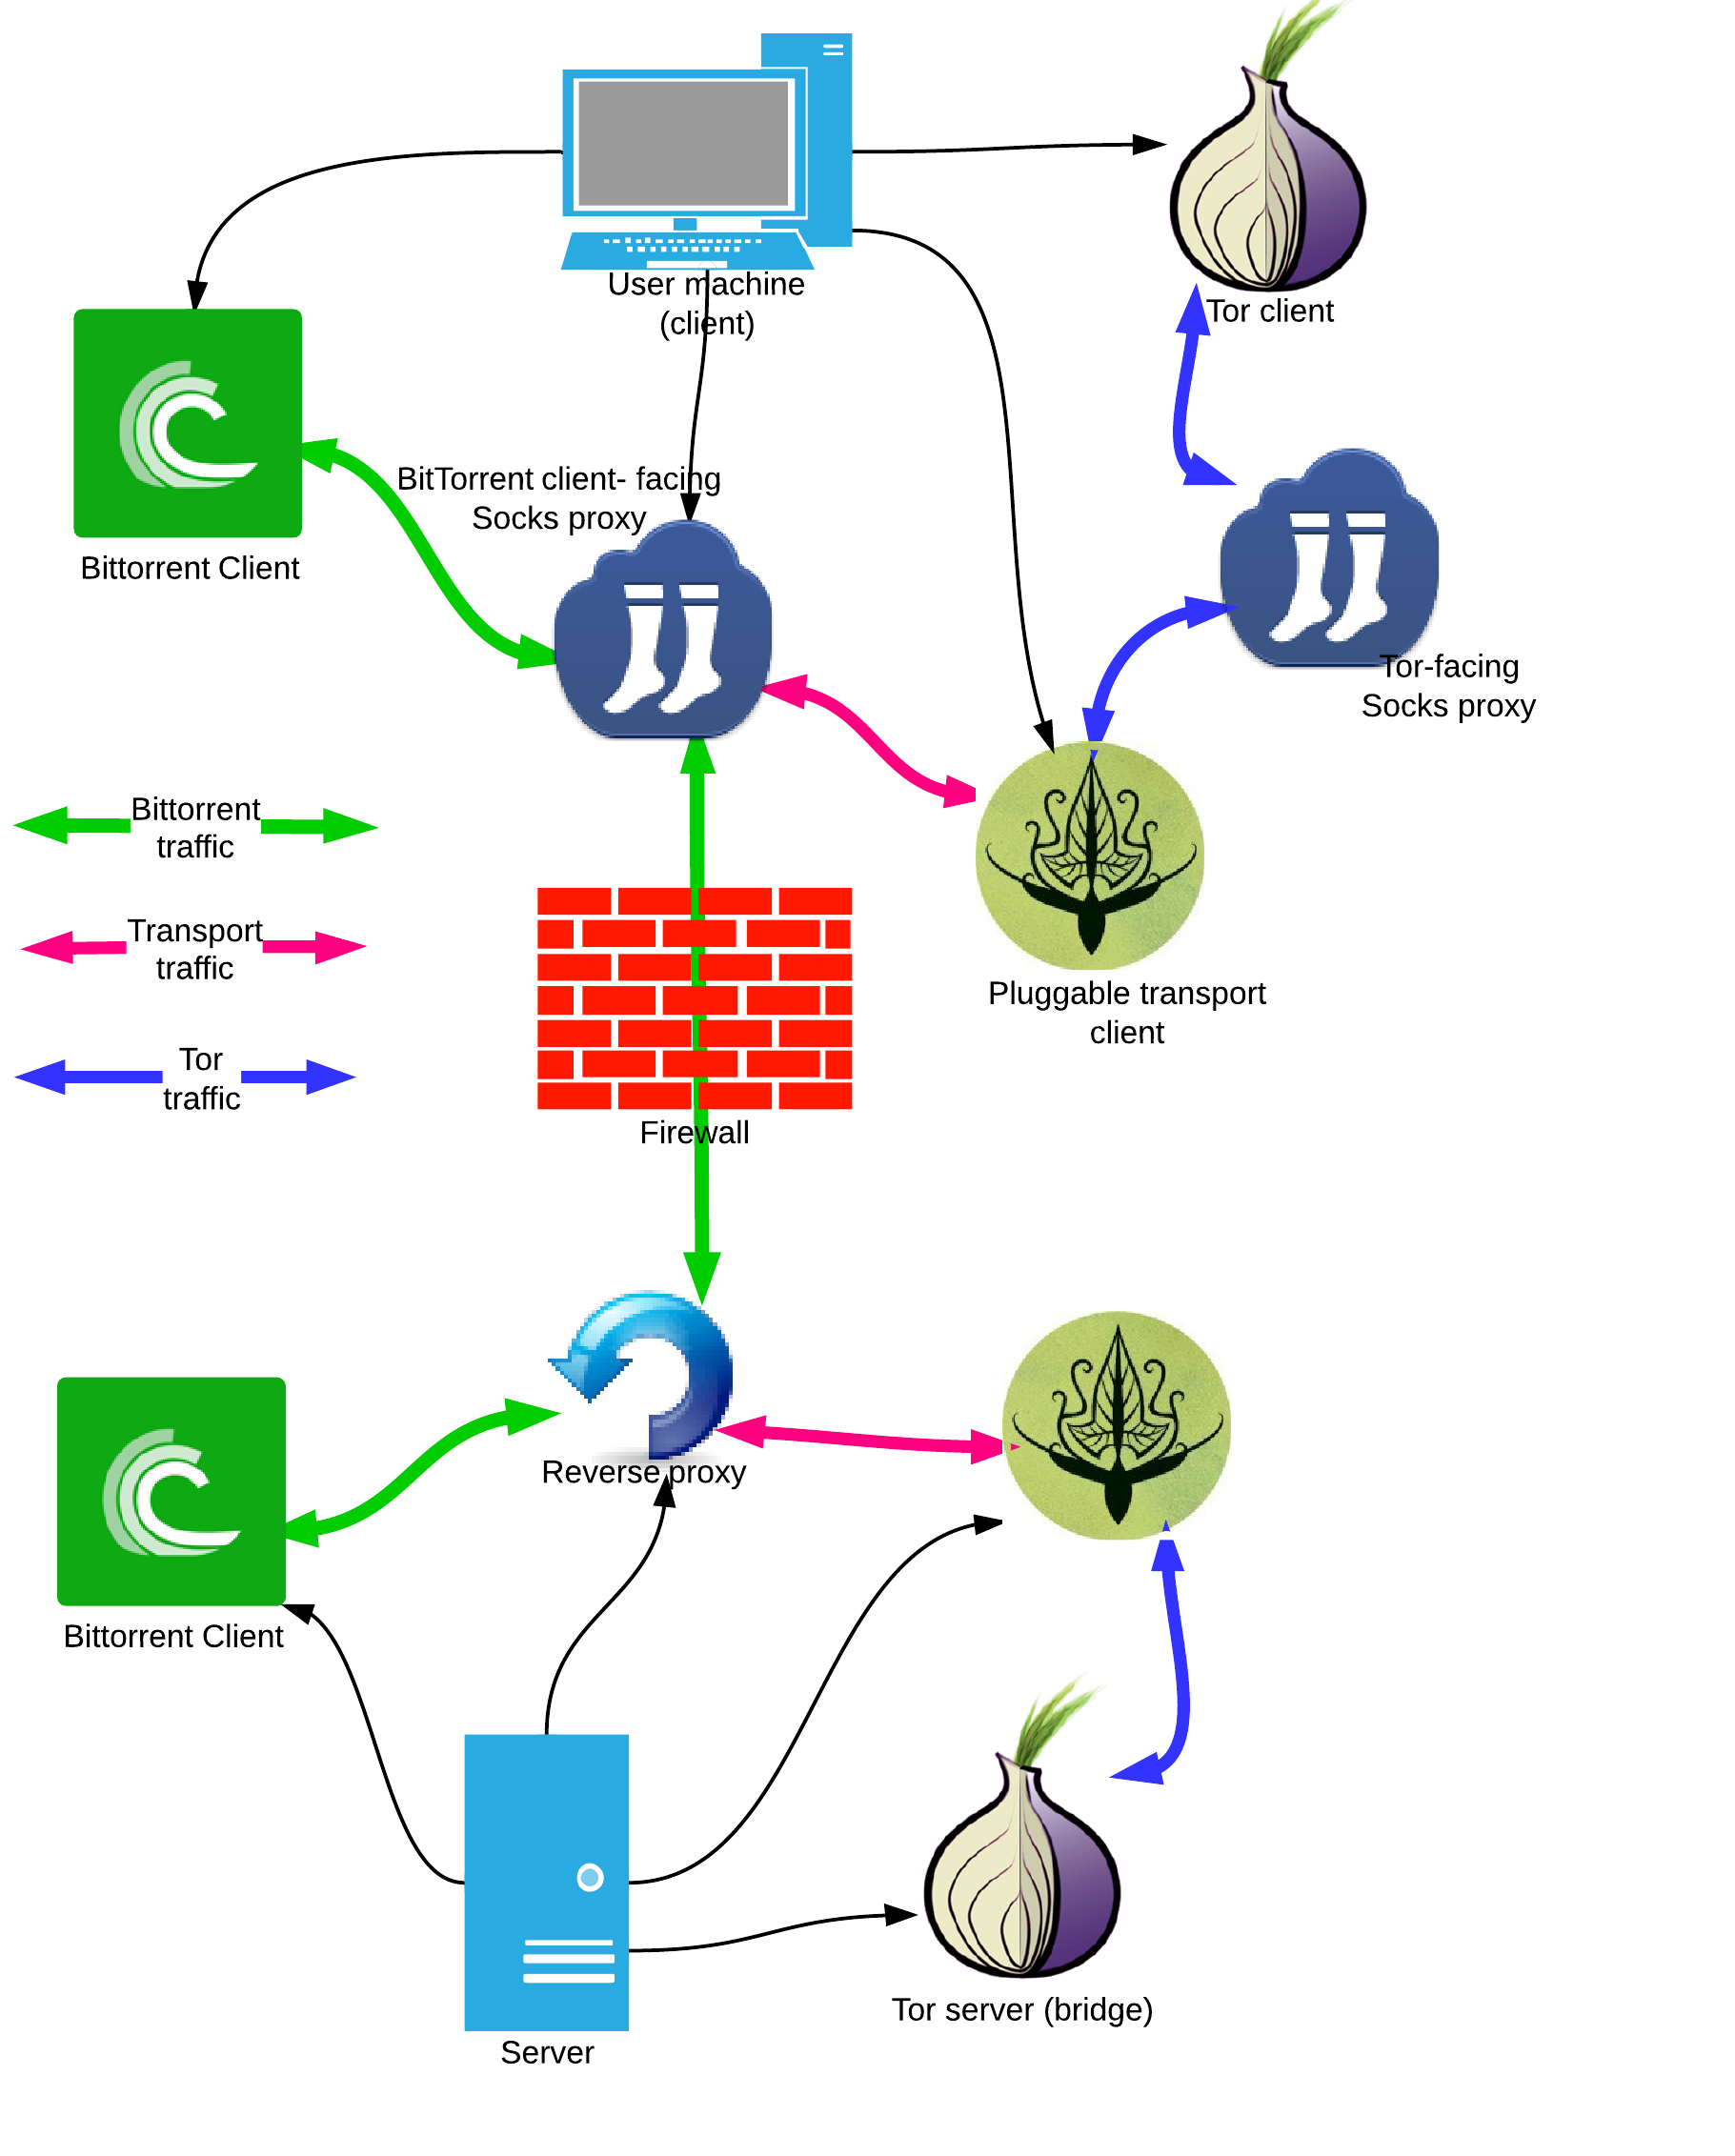
\includegraphics[scale=0.23]{FuinSystemArchitecture}
\end{center}
 \caption{System overview}
 \label{fig:system_architecture}
 \end{figure}

\subsubsection{The life of a Tor data byte}

In order to better understand how the whole data channel works we will describe step by step, the lifetime of a data byte after it is sent by the Tor client and until it reaches the Tor bridge. This is described assuming the whole connection has already been established and intiation/handshaking completed. Note that for all other purposes the data is reasoned about as a stream, but we look at a single byte to understand the flow.

A byte is sent by the Tor client process to the Tor bridge. It is proxied to a localhost socks proxy that the Tor client is configured to use. It is then picked up by the PT client process who controls the socks proxy. The PT process then waits for a BitTorrent piece to take the byte over the network. The PT process runs another socks proxy facing the Bittorrent client. It can thus see all incoming and outgoing BitTorrent messages going through a connection \textit{initiated} by its BitTorrent client. When a piece message created by the \textit{local} BitTorrent client is seen by the PT process, it tampers with its contents, removes its old content (a part of the file it was transporting) and inserts the byte encrypted.  

The BitTorrent message travels across the network through the adversary's firewall (hopefully unseen, unheard) and reaches the server machine. It is then proxied through the reverse proxy standing in front of the BitTorrent client living on the server side. This reverse proxy is owned by the PT server process which looks at all incoming piece messages to see if they are holding transport protocol payload. When the travelling byte's message reaches it, it decrypts the whole payload, extracts the byte, sends the piece further on to the server-side BitTorrent client. It then sends the byte through the open Extended ORPort connection to the Tor bridge process running locally.

In a similar, but not identical way (since there is assimetry between the client and server) a byte travels from the Tor bridge to the Tor client.

\subsubsection{BitTorrent client interaction}

A critical design choice of this project is that to use a \textit{real} BitTorrent client to generate BitTorrent traffic between the client and the server. This choice was made in order to obtain an authentic BitTorrent traffic pattern that is indistinguishable from genuine traffic. However, this came with the tradeoff of a more complex implementation.

As we saw above, using a BitTorrent client to generate transport traffic involves proxying its connection with a socks proxy on the client (because it's an outgoing connection) and a reverse proxy on the server-side (because it is an incoming connection). Furthermore, in order to correctly read and tamper with the BitTorrent messages, the entire stream of the BitTorrent connection is parsed and then serialized back on its way out of the proxy. 

 The BitTorrent client in use needs to be controlled by the PT process. Therefore, the client needs to support the following actions in an automated fashion (i.e. exposing a network API/command line interface):

\begin{itemize}
\item socks proxy configuration
\item Adding a torrenfile/magnet link
\item control per torrent file pausing, resuming, upload/download speed, adding peers
\end{itemize}

To fully achieve the goal of creating indistinguishable BitTorrent traffic, the sum of the usage share of the BitTorrent clients employed by the system needs to be high. To undestand this, think about the extreme situation in which the system uses only one particular obscure BitTorrent client with a 0.1\% market share, in which case the adversary can focus his detection efforts on the connections which involve only those particular clients, as deduced from the plaintext handshake of the BitTorrent protocol.

Given the requirement above, the system is designed to support multiple types of BitTorrent clients which in turn are required to support the features mentioned above to allow for control and proxying. For this purpose, a general BitTorrent client interface was designed, which requires implementations for each client. The current codebase contains control modules for the UTorrent client and the Deluge client. The UTorrent client  was chosen since it comes up as being either the first or second most popular client based on information collected by trackers, while the Deluge client was selected because its deluged daemon is ver configurable allowing for fine-grained control, making it the best fit for initial prototyping and demos. 

The following snippet shows the Haskell  data type associated with a BitTorrent client connection: 

\begin{lstlisting}
data TorrentClientConn
  = TorrentClientConn {
       addMagnetLink :: (MonadTorrentClient m) => String -> m (),
       addTorrentFile :: (MonadTorrentClient m) => String -> DB.ByteString -> m TorrentHash,
       listTorrents :: (MonadTorrentClient m) => m [Torrent],
       pauseTorrent :: (MonadTorrentClient m) => TorrentHash -> m (),
       setProxySettings :: (MonadTorrentClient m) => [ProxySetting] -> m (),
       connectPeer :: (MonadTorrentClient m) => TorrentHash -> HostName -> PortNumber -> m ()
\end{lstlisting}

\subsection{Tools}

The tools involved in developing the system

\subsubsection{Programming language}

When choosing the programming language for the project the main criteria were:

\begin{itemize}
\item is high-level
\item favors code reuse
\item favors correctness and security
\item has reliable network, concurrency, cryptography libraries
\item the language toolchain (compiler/interpreter, profiler) allow you to produce efficient code in terms running time and space performance
\end{itemize}

Haskell is the programming language of choice for this project. Haskell is a high-level purely functional language that is advertised as being good for the rapid development of correct, robust software. It's type system is both flexible and powerful allowing you to write code that is concise and reusable while at the same time subjected to a great deal of compile time checks.

Atlhough not a requirement, the fact that the language allows you to write pure computations (no side-effects, equivalent of mathematical functions) combined with the strong compile time checks makes it much  easier to write correct code. Whenever it is the case below, I will emphasize when a particular code component has been implemented in a pure fashion to facilitate testability and achieving correctness.

The fact that the Haskell toolchain allows for writing of performant network applications has been proved empirically by the creation network applications such as the Warp HTTP web server whose performance exceeds that of other modern systems (node, tornado, php) \citep*{web:warpCrossBenchmark}.

As for the availability of libraries, the choice of programming language was not the correct one in terms of prototyping and quick results. I believe Python would have been the obvious correct choice. If I were to choose Python the following libraries/modules would have been available:

\begin{itemize}
\item Twisted networking engine 
\item socks/reverse proxy server
\item Extended OrPort protocol  
\item BitTorrent protocol parser
\item REncode
\item deluged RPC API 
\item uTorrent RPC API
\end{itemize}

The parsing, encoding and protocol modules above needed equivalent implementations in Haskell.  Haskell doesn't have a direct equivalent of Twisted, namely a framework for writing custom network applications. However, one can argue that by combining existing Haskell libraries you can get equivalent functionality with not much extra boilerplate code, as we shall see in the libraries section.

Not only this but Python, being high-level, dinamically typed, and generally well designed, is a very good choice for prototyping and writing programs whose final shape is not known and where signficant design changes happen while implementing. It can be argued that this was the case for this system.

Two other aspects which greatly affected productivity but were not amongst the main considerations when choosing the programming language are \textit{familiarity} and \textit{learning curve}. I was moderately familiar with Python and it has a short learning curve, while I was a beginner Haskell programmer and the language has a significantly longer learning curve. Thus, a lot of the time spent on the project was invested in learning Haskell.

Having said that Python would have been the correct choice for prototyping, I would argue that Haskell is the long term correct choice, since it meets the other stated criteria and the minor lack of libraries is something that can be compensated by just investing development effort.

\subsubsection{Libraries}

On the flip side, the Haskell libraries that are available are reliable and efficient and superior to libraries in other languages solving similar problems.

Based on importance in the project, the following libraries are worth mentioning:

\begin{itemize}
\item  Control.Concurrent - offers explicit concurrency abstractions. 
\item Control.Concurrent.STM - software transactional memory implementation
\item Data.Conduit -  library for handling streams of data
\item Data.Attoparsec - library for writing parsers in a concise, declarative way
\end{itemize}

\myparagraph{Control.Concurrent}

I used this library for concurrent handling of requests and tasks.

The main primitive of the library is forkIO which allows you to spawn a thread that is sent off to perform a computation. As of GHC 6.12, that thread is not an OS level thread, but a user-space green thread, which means many (read: millions) of such threads can be created without being concerned with expensive creation, per thread memory consumption, context switching and finalization. These threads run in what is called an event loop.

The nice thing about the Haskell implementation of green threads is that for the user (programmer) the IO actions of green threads are still expressed naturally in the IO monad with no changes required. Other environments supporting green threads such as NodeJS, Dart or Python Twisted force you to write code in a continuation-passing-style with a callback or defferred object for each IO action. 

The following code snippet illustrates the loop handling new connections in the proxy module. Each new connection is handled independently by the handleConn function.

\begin{lstlisting}
loop config serverSock
  = forever $ accept serverSock >>= liftIO . forkIO . (handleConn config)
\end{lstlisting}

Nonetheless, the underyling GHC implementation for threads is using an even-driven model which makes efficient use of all machine cores, all being abstracted away from the user (the programmer). It can be said that Haskell makes the best of both worlds (the event driven concurrency and threaded concurrency model).
\myparagraph{Control.Concurrent.STM}

This library provides safe access of shared memory where all accesses are modelled as transactions (hence the name).

My main use case for this library are message channels. In order for the threads to do useful work together, they communicate by sending messages to each other through channels. Although implemented in the STM library, channel communication should be understood as "no-shared-memory" way of communicating where a thread pushes a message inside a channel and another thread reads it from that channel.

The next code snippet shows how the socks proxy thread notifies the PT client thread that it has finished initializing the proxying of a BitTorrent connection by sending a message through a control channel.
\begin{lstlisting}
-- proxy initialization function
liftIO $ atomically $ writeTChan control Done
-- ...
-- the PT client thread 
 completion <- liftIO $ timeout btConnInitTimeout
		                   (liftIO . atomically . readTChan $ control)
 when (completion == Nothing) $ throwError "bittorrent connection start timeout"
\end{lstlisting}

\myparagraph{Data.Conduit}

The conduit library is used for modular and efficient handling of data streams. I used it for handling the data streams of the proxies and for processing the stream of incoming and outgoing transport protocol messages  in a pipeline-like fashion.

The next snippet shows the how the stream of incoming BitTorrent Piece payloads is handled in order to be transformed in transport protocol messages:

\begin{lstlisting}
streamIncoming msgChan payloadChan decrypt =
   (chanSource payloadChan)
   $= map decrypt --attempt to decrypt all incoming payload
   $= filter (/= Nothing) $= map fromJust -- filter the succesfully decrypted ones
   $= conduitParser parseTransportMessage -- parse the messages
   $$ chanSink msgChan -- send them down the message channel
\end{lstlisting}

Notice how this style of coding isolates the reading and writing of data IO actions (in this case reading/writing channels) from the logic of the transformations on the stream which are pure computations that can be tested separately.

I also used the Data.Conduit library for a more unconventional purpose: writing network protocols. A network protocol was modelled as a conduit that takes as an input a stream of bytes and produces a stream a bytes or a final result. The next snippet illustrates the data types and the function used to run the protocol:

\begin{lstlisting}
type ProtocolConduit a = (MonadNetworkProtocol m) =>
					 Conduit ByteString m (ProtocolOutput a)
data ProtocolOutput a = ProtoData ByteString | FinalResult a
runProtocol :: (MonadNetworkProtocol m, MonadIO m) =>
			(ProtocolConduit a) -> Socket -> m (Maybe a)
runProtocol protocol sock
  = (sourceSocket sock) =$ protocol $$ (sinkSocketWithResult sock)
\end{lstlisting}

Thus, to implement the the ExtendedOR Port initialization protocol, one needs to implement a Conduit computation with the ProtocolConduit signature.

This achieves the following: the protocol logic is implemented as a \textit{pure computation}  in the form of a stream transformation decoupled from the IO actions of reading and writing to network sockets.

\myparagraph{Data.Attoparsec}
Attoparsec was the parser library of choice used for parsing the message streams of all the implemented protocols because the library was build with this particular task in mind.

The library allows for expressing parsing functions in a concise, pure manner as shown in the following snippet for parsing the socks5 handshake message:

\begin{lstlisting}
parseHandshake :: Parser Handshake
parseHandshake = do
  versionByte <- anyChar
  methodCount <- fmap ord anyChar
  methods <- replicateM methodCount anyChar
  return $ Handshake versionByte methods
\end{lstlisting}

\subsection{Code structure}

The codebase was developed with a focus on building reusable modules. At this stage the code requires more refactoring work, documentation and optimization to meet Hackage standards, but as it stands it is clearly structured and abstract enough to be reusable.

The user facing Haskell modules are the Client and Server modules. The next snippets give a feel about how to use these modules for communicating through a BitTorrent camouflaged channel (no Tor integration just yet):

\begin{lstlisting}
-- Client interface

   transport <- Client.init socks5ProxyPort torrentClientConnection
   let info = serverInfo clientEncyption serverTorrentFile serverSockAddr
   conn <-  Client.makeConn transport info
   connectionPut conn "why hello there"
   response <- connectionGetChunk conn
\end{lstlisting}

\begin{lstlisting}
-- Server interface

{-
receiverPublicPort - the publicly advertised BitTorrent port for incoming connections
receiverPrivatePort - the port at which the BitTorrent reverse proxy listens and where all BT traffic is redirected on
-}
Server.run echoHandleConn receiverPublicPort
					   receiverPrivatePort
				           serverEncryption
					   torrentClientConnection	
echoHandleConn conn
  = forever $ (connectionGetChunk  conn) >>= (connectionPut conn)
\end{lstlisting}

The rest of the modules are auxilliary modules but many are standalone pieces of code that can be integrated as individual packages in Hackage.

\begin{itemize}
\item NetworkProtocol - module defining an interface for writing and running network protocols as Conduits
\item Proxy - customizable proxy with a hook in connection initialization and Conduit hooks into the incoming/outgoing traffic; has logic for running socks proxies and reverse proxies
\item Extended OrPort protocol  - Tor protocol for connecting a pluggable transport to the Tor bridge
\item BitTorrent Message  - parser and serializer for the stream of BitTorrent messages. implemented using Attoparsec and the Data.Binary package
\item BitTorrentClient - module defining a general interface for BitTorrent client communication
\item deluged RPC API - library for communicating with the deluged daemon from Haskell
\item uTorrent Web API - library for communicating with the uTorrent server from Haskell
\item REncode - library for an encoding algorithm of loosely structured data. It is the Deluge project's more optimized version of the original BEncode encoding created for the BitTorrent project 
\item Stream - contains data stream handling functionality common between the Server and the Client
\item Utils - module containing miscellaneous useful functions
\end{itemize}

\subsection{Tor integration}

The system runs as an externally managed Tor pluggable transport and doesn't make use of any of the existing Tor modules/frameworks for plugabble transports.

Many of the other Tor pluggable transports (StegoTorus, ScrambleSuit, Dust) make use of the Tor obfsproxy  framework for developing pluggable transports. For developing this particular pluggable transport the obfsproxy framework isn't flexible enough. The reason is that obfsproxy handles the connection to the Tor server and client itself allowing you to "plug in" the transport logic in the middle, while in the case of our system there is no direct connection between the Tor client and bridge. The only connection over the network is the Bittorrent connection.

As stated previously, the choice of programming language prevented any code reuse since obfsproxy and most Tor plugabble transports are developed in Python, C++ or more recently Go(meek). However, by developing the current solution we set foundation for the development of Tor pluggable transports in Haskell: the custom socks server module and the ExtendedORPort connection are the ncessary glue to handle Tor client and Tor bridge connections, respectively.

 

\section{Evaluation}

The evaluation of this project is tricky. Ideally we would like to answer the question of whether this covert channel does good a good job at avoiding filtering by censorship firewalls. Testing in a real life situation is irrelevant, because at the time of writing, no detection method is yet deployed by adversaries, since it is a completely new covert channel and adversaries will make no effort to block it until it is deployed at scale by the Tor network.

We would want to know what is the detection rate of the pluggable transport what resources are needed to perform detection and what are performance costs of the covert channel (the resulting bandwidth).

A way of evaluating it is for the author to take up the role of the attacker and devise attacks to measure their effectiveness. Based on the design of my pluggable transport, I will be creating packet analysis techniques meant to detect whether a bittorrent connection hides Tor traffic. I will further evaluate the costs of deploying and running such as solution at scale by the adversary. 

Furthermore, expanding on the idea of playing the role of the adversary, I would post my solution to security communities and challenge them to hack it. I was planning to organize a local university event as well in the form of a hackathon and participants will be ranked according to their detection success rate and perhaps computational resource utilization and awarded prizes accordingly. The main goal is to get the designed reviewed and hacked to make it as bulletproof as possible or maybe, if it proves fundamentally flawed, discard it.

\subsection{Theoretical evaluation}

\subsection{Practical evaluation}

\section{Conclusion}

\section{Further work}


\section{Annexes}


C code for ballparking how much computation can be performed in 1 microsecond.
Compiled with g++ -Ofast.
\begin{lstlisting}
#include <stdio.h>
#include <sys/time.h>


long long current_timestamp() {
    struct timeval te; 
    gettimeofday(&te, NULL); // get current time
    return te.tv_usec;
}

int compute(int x) {
  return (x + 1) *(x + 1);
}

int main() {
  int s = 0;
  long long start = current_timestamp(); 
  int n = 10000;
  char a[n];
  for (int i = 0; i < n; i++)
    s += compute(a[i]);
  printf("%llu hello %x", current_timestamp() - start, s);
}
\end{lstlisting}

\bibliographystyle{plainnat}
\newpage
\bibliography{references}

\end{document}


